\section{截面诊断}
基础合格池U已应用历史ST/PT和入场资格筛选；F为U中可构造BP的股票；S为F中行业与市值控制变量可用的分析样本。覆盖率统一定义为F/U。

\subsection{一级行业分布}
\Needspace{185mm}
\begin{figure}[H]\centering
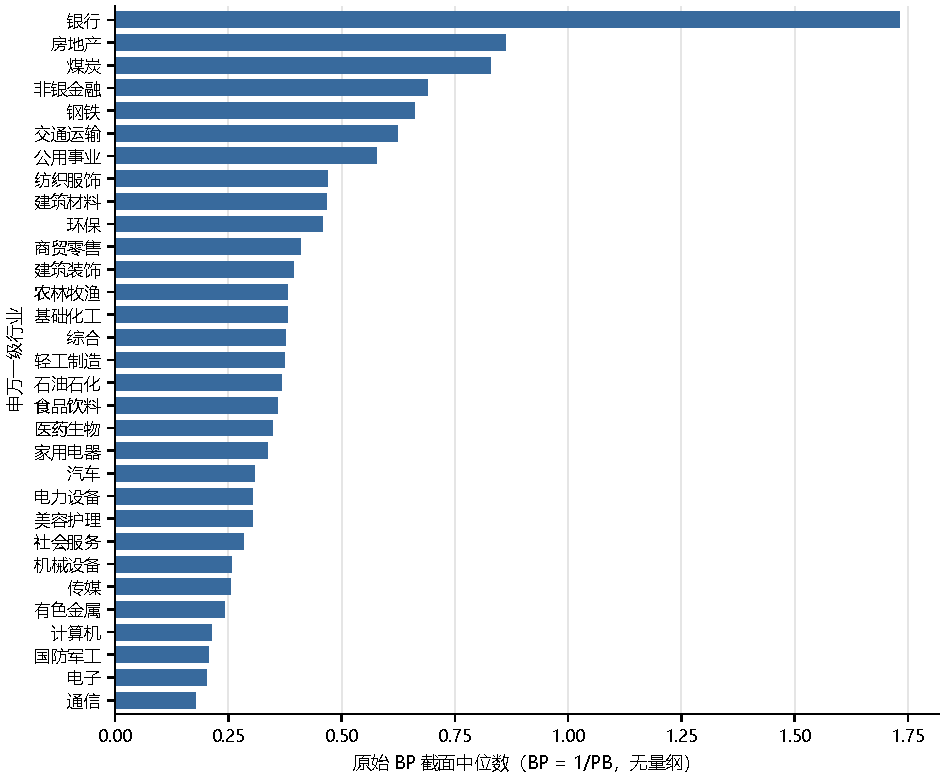
\includegraphics[width=.8\linewidth]{figures/industry_median.pdf}
\caption*{\textbf{图A　最新截面的行业BP中位数}\ 2026-01-30；使用正且有限PB的F样本；覆盖31个一级行业。横轴为原始BP，不是中性化残差。}
\end{figure}

最新截面共5273只F股票、31个一级行业。银行BP中位数为1.732，通信为0.177，前者约为后者的9.8倍。房地产和煤炭也处于较高区间。这种行业差异支持在比较股票之前控制行业；不能把银行高BP本身解释为银行股票具有更高预测收益。综合行业在本截面仅15只，仍展示中位数，但不据此认定其行业分层可靠。

\Needspace{115mm}
\subsection{BP与规模的关系}
\Needspace{85mm}
\begin{figure}[H]\centering
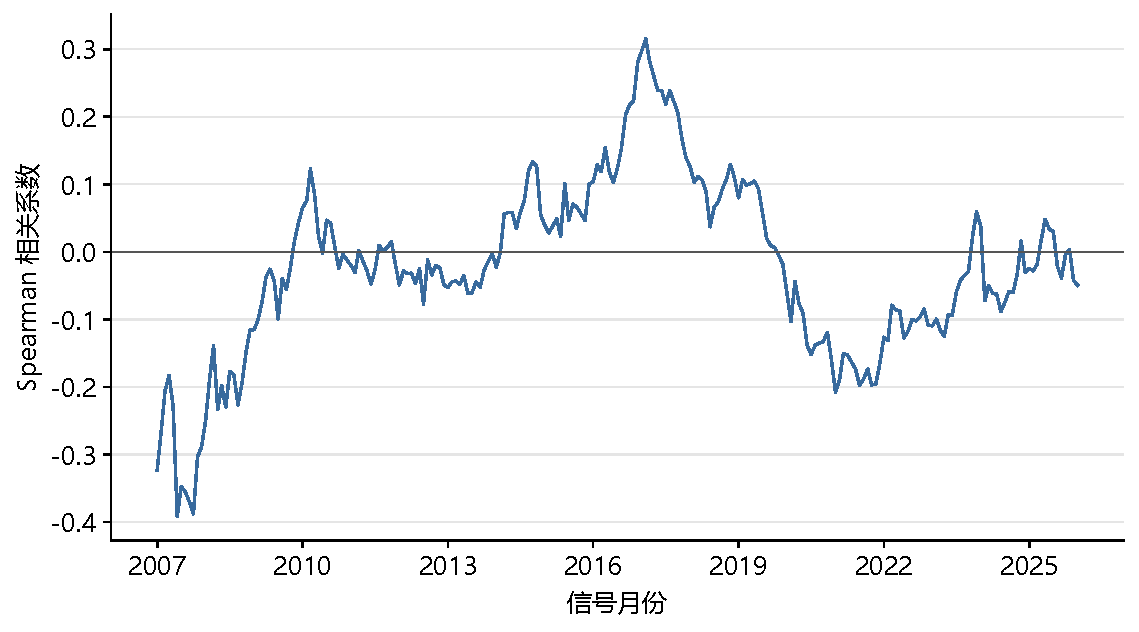
\includegraphics[width=.87\linewidth]{figures/size_correlation.pdf}
\caption*{\textbf{图B　原始BP与对数总市值的截面相关}\ 2007-01至2026-01，共229个信号月；逐月计算Spearman相关，未按未来收益筛选。}
\end{figure}

229/229个信号截面均可计算，相关系数均值为-0.0228；与均值同为负号的月份为136/229（59.39\%），正号为93/229。均值较小并不表示每月都与规模无关，图中方向曾发生反转。因此保留逐期规模控制，且不把中性化后的低相关倒写为原始BP无规模关联。

\Needspace{100mm}
\subsection{覆盖度与样本流转}
\Needspace{85mm}
\begin{figure}[H]\centering
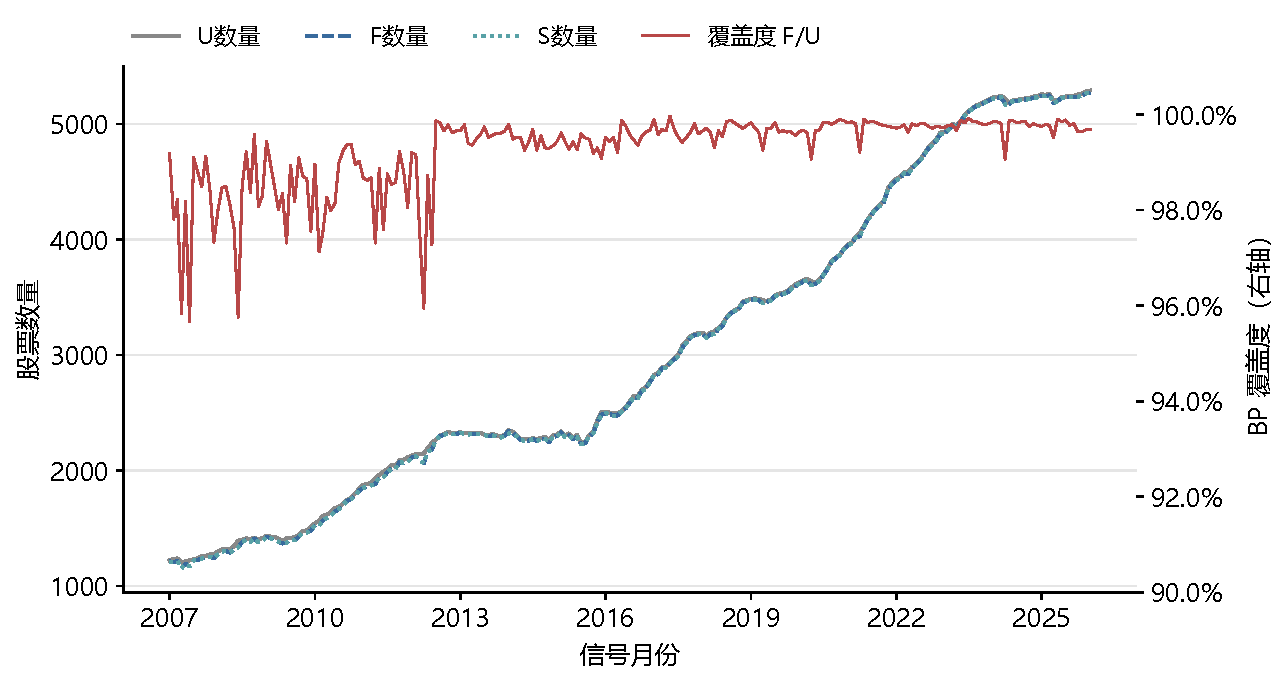
\includegraphics[width=.87\linewidth]{figures/D1.pdf}
\caption*{\textbf{图D1　合格样本与BP覆盖度}\ 全部 A 股；229个信号月。数量读左轴，覆盖率F/U读右轴；收益检验只使用其中228个完整持有期。}
\end{figure}

全部 A 股各月F/U介于95.66\%与99.97\%。最新截面U=5,290、F=S=5,273，覆盖度为99.68\%。229期累计U与F之差为3,602个股票期观测，其中估值整行缺失2,660、PB字段缺失942、非有限0、零值0、负值0。缺失不能统一解释为负净资产；ST/PT和入场不合格已在U之前过滤，不进入覆盖率分母。覆盖度较高仅支持数据可用性，不等于预测有效性。

